\documentclass[11pt,oneside]{article}
%\documentclass[oneside,10pt]{book}

\title{ {\huge \sc Linear programming tutorial} }
\author{Ivan Savov}
\usepackage{amsthm,amsmath,amssymb,amsfonts,latexsym}
\usepackage{graphicx}
\usepackage{hyperref}


%%%%%%%%%%%%%%%%%%%%%%%%%%%%%%%%%%%%%%%%%%%%%%%
% STEP 1: Choose the true/false values for   DRAFTMODE
%%%%%%%%%%%%%%%%%%%%%%%%%%%%%%%%%%%%%%%%%%%%%%%
\usepackage{ifthen}
\newboolean{DRAFTMODE}				% if PROOFREADING=true:
\setboolean{DRAFTMODE}{true}			%   10pt, dblspaced, 8.5'' x 11'' paper



%%%%%%%%%%%%%%%%%%%%%%%%%%%%%%%%%%%%%%%%%%%%%%%
% STEP 2: done!
%%%%%%%%%%%%%%%%%%%%%%%%%%%%%%%%%%%%%%%%%%%%%%%



%%%%  LAYOUT SETTINGS   %%%%%%%%%%%%%%%%%%%%%%%%%%%%%%%%
\ifthenelse{\boolean{DRAFTMODE}}{			
    %  PROOFREADING  SETTINGS %%%%%%%%%%%%%%%%%%%%%%%%%%%%%%    
   %
%\usepackage{setspace} 
%\linespread{1.3}
	
% LOTS OF SPACE
%    \usepackage{setspace} 
%    \linespread{2}
%    \usepackage[papersize={8.5in,11in},margin=3cm]{geometry}

	% Same-width-as-final proofreading format
         \usepackage[ papersize={8.5in,11in}, verbose,
                                headsep=0.5cm, tmargin=1.7cm,          	
                              lmargin= 3.5cm,rmargin= 3.5cm, 
                                bmargin=1.7cm, footskip=0.7cm]{geometry}
                                
	%% book-like
	%\usepackage[     papersize={5.5in,8.5in}, verbo	se,
	%                                headsep=0.3cm, tmargin=1.3cm, lmargin=2.25cm,
	%                                rmargin=1.15cm, bmargin=1.5cm, footskip=0.6cm]{geometry} 
    
}{
    %  FINAL  SETTINGS %%%%%%%%%%%%%%%%%%%%%%%%%%%%%%%%%%%%
%    \usepackage{answers}							% use for final version
    \usepackage[     papersize={5.5in,8.5in}, verbo	se,
                                headsep=0.3cm, tmargin=1.3cm, lmargin=2.05cm,
                                rmargin=1.35cm, bmargin=1.5cm, footskip=0.6cm]{geometry}
}
%%%%%%%%%%%%%%%%%%%%%%%%%%%%%%%%%%%%%%%%%%%%%%%

	\usepackage{fancyhdr}
	\usepackage{textcase}

	\fancypagestyle{plain}{
	    \fancyhf{}
	    %\fancyfoot[RO,LE]{{\footnotesize \thepage}}
	    \renewcommand{\headrulewidth}{0pt}
	    \renewcommand{\footrulewidth}{0pt}
	    \fancyfoot[C]{\footnotesize\thepage}	    
	}

\pagestyle{fancy}
\fancyhf{}
\fancyhead{} 

\makeatletter
\renewcommand{\sectionmark}[1]{\markright{\thesection~~\MakeTextUppercase{#1}}}
\makeatother

\fancyhead[LE]{\footnotesize\thepage}
\fancyhead[CE]{\footnotesize\sc \leftmark}	 % \nouppercase
\fancyhead[CO]{\footnotesize\sc \rightmark}
\fancyhead[RO]{\footnotesize\thepage} 

\renewcommand{\headrulewidth}{0pt} % no line plz

 
%   below is some really useful code for automatically inserting the version
%   number below the title of the paper. This way we know which version we
%   have printed out and can see what has changed since then.
%   (uncomment one level to activate -- probably will only work on your Mac)
%
%%================================================================================
%% CALL OUT TO SHELL to get current hg revision number 
\newread\myinput
% We use '\jobname.temp' to create a uniquely-named temporary file
\immediate\write18{git log -l1 | grep "^commit" | cut -c-14 > '\jobname.temp'}
\immediate\openin\myinput=\jobname.temp
% The group localizes the change to \endlinechar
\bgroup
  \endlinechar=-1
  \immediate\read\myinput to \localline
  % Since everything in the group is local, we have to explicitly make the
  % assignment global
  \global\let\gitrevisionnumber\localline
\egroup
\immediate\closein\myinput
% Clean up after ourselves
\immediate\write18{rm -f -- '\jobname.temp'}
%\hgrevisionnumber used to be \myresult
%\dosomething{\myresult}
% via http://stackoverflow.com/questions/2671079/how-can-i-save-shell-output-to-a-variable-in-latex
%%================================================================================




\usepackage{wasysym}
\usepackage{pifont}
\usepackage{xcolor}
\usepackage{tikz}
\usetikzlibrary{arrows}
\usetikzlibrary{patterns}
\usetikzlibrary{decorations}
\usetikzlibrary{matrix}
\usetikzlibrary{snakes}
\usetikzlibrary{calc}
\usepackage{subfigure}



% QUANTUM
\newcommand{\bra}[1]{\langle #1|}
\newcommand{\ket}[1]{|#1 \rangle}
\newcommand{\braket}[1]{\langle #1 \rangle}
\newcommand{\ketbra}[1]{\ket{#1}\bra{#1}}
\newcommand{\ketb}[2]{\ket{#1}\bra{#2}}
\def \Tr{\textup{Tr}}
\def \c{\mathbb{C}}
\newcommand{\sfT}{{\mathsf{T}}}			% Transpose


\theoremstyle{definition}
\newcommand{\be}{\begin{equation*}}
\newcommand{\ee}{\end{equation*}}

% Info panels 
\usepackage{framed}
\usepackage{tensor}
\usepackage{bbm}							% for the identity matrix \mathbbm{1}  
\usepackage{mathtools}   % for bsmallmatrix 
\usepackage{enumitem}


\newcommand{\thrmname}[1]{\textbf{#1}}





\begin{document}


\maketitle 

\vspace{-1cm}
\noindent

{ \center
	git \gitrevisionnumber 

}

\vspace{1cm}

\setcounter{tocdepth}{2}
\setcounter{secnumdepth}{2}
\tableofcontents

\vspace{1cm}

\section{Linear programming}
\label{applications:linear_programming}

	In  the early days of computing, 
	computers were primarily used to solve optimization problems
	so the term ``programming'' is often used to describe optimization problems.
	\emph{Linear programming} is the study of linear optimization problems that involve linear constraints.
	%	linear programming, quadratic programming, semidefinite programming.	
	Optimization problems play an important role in many business applications:
	the whole point of a corporation is to constantly optimize profits,
	subject to time, energy, and legal constraints. 
	%	their operations within budgetary, time, and production constraints. 
	
	Suppose you want to maximize the quantity $g(x,y)$ subject to some constraints on the values $x$ and $y$.
	To maximize $g(x,y)$ means  to find the values of $x$ and $y$ that make $g(x,y)$ as large as possible.
	Let's assume the \emph{objective function} $g(x,y)$ represents your company's revenue,
	and the variables $x$ and $y$ correspond to monthly production rates of ``Xapper'' machines and ``Yapper'' machines.
	You want to choose the production rates $x$ and $y$ that maximize revenue.
	If the revenue from each Xapper machine is \$3000 and the revenue from each Yapper machine is \$2000,
	the monthly revenue is described by the function $g(x,y) = 3000x +  2000y$. 
	%	This is the objective function.

	Due to the limitation of the current production facilities,
	the rates $(x,y)$ are subject to various constraints.
	We'll assume each constraint can be written in the form $a_1x+a_2y \leq b$.
	%
	The maximum number of Xapper machines that can be produced in a month is three, written $x\leq3$.
	Similarly, the company can produce at most four Yapper machines, denoted $y \leq 4$.
	Suppose it takes two employees to produce each Xapper machine and one employee to produce each Yapper machine.
	If the company has a total of seven employees,  % TODO: change phrase to remove conditional If...
	the human resources limits impose the constraint $2x+y \leq 7$ on the production rates.
	Finally, logistic constraints allow for at most five machines to be shipped each month, which we write as $x+y \leq 5$.

	This production rate optimization problem can be expressed as the following \emph{linear program}:
	\begin{align*}
		\max_{x,y} 	g(x,y) \ &=\  3000x  \, + \,  2000y, \\  % \qquad [\$], 	\\ 
	\intertext{subject to the constraints}
				x 		\ &\leq \		3,	\\
					y	\ &\leq \	 	4,	\\
				2x	+ y	\ &\leq \	 	7,	\\
				x 	+ y	\ &\leq \	 	5,	\\
				x \geq 0, 	& \quad  	y \geq 0.
	\end{align*}
	Each of the inequalities represents one of the real-world production constraints.
	We also included the non-negativity constraints $x \geq 0$ and $y \geq 0$ to show
	it's impossible to produce a negative number of machines---we're not doing an accounting scam here,
	this is a legit Xapper--Yapper business.
	
	
	On first hand the problem looks deceptively simple.
	We want to find the coordinates $(x,y)$ that maximize the objective function $g(x,y)$,
	so we can simply find the direction of maximum growth of $g(x,y)$ and go as far as 
	possible in that direction.
	
	Rather than attempt to plot the function $g(x,y)$ in three dimensions,
	we can visualize the growth of $g(x,y)$ by drawing \emph{level curves} of the function,
	which are analogous to the lines shown on topographic maps.
	Each line represents some constant height: $g(x,y)=cn$, for $n \in \{0,1,2,3, \ldots \}$.
	Figure~\ref{fig:linear_programming_level_curves_gxy} shows the level curves
	of the objective function $g(x,y)=3000x +  2000y$ at intervals of $3000$.
				
		\begin{figure}[htb]
		\begin{center}
		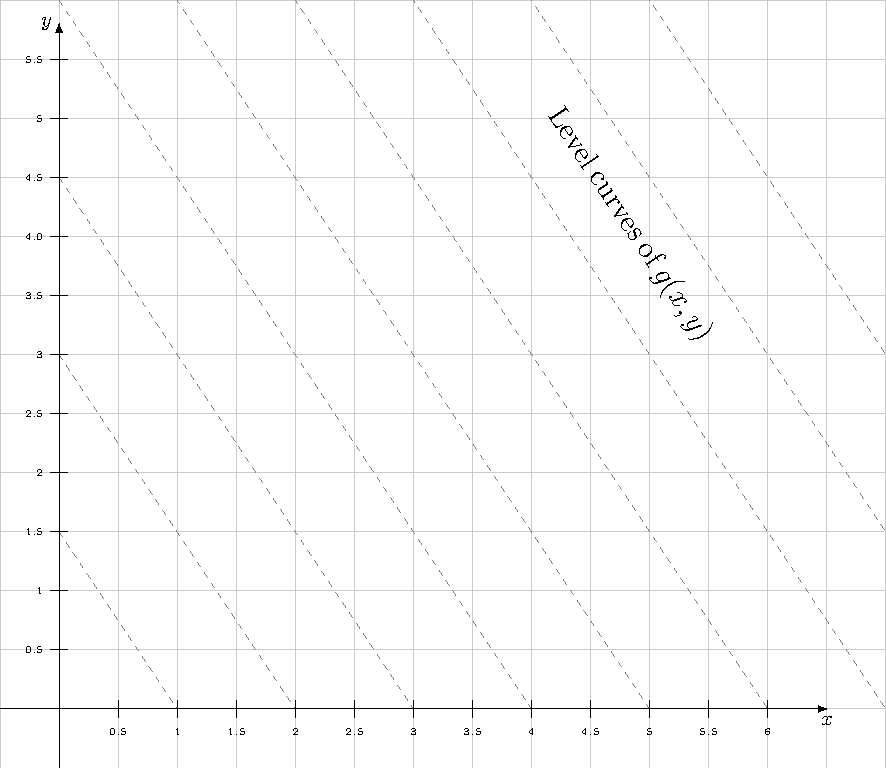
\includegraphics[width=0.6\textwidth]{figures/linear_algebra/linear_programming_level_curves_gxy.pdf}
		%TODO: annotate each line with g value 
		\end{center}
		\vspace{-6mm}
		\caption{The objective function $g(x,y)=3000x +  2000y$ grows with $x$ and $y$. 
				The direction of maximum growth is $(3,2)$---if you think of $g(x,y)$ 
				as describing the height of a terrain, 
				then the vector $(3,2)$ points uphill.
				The dashed lines in the graph represent the following \emph{level curves}:
				$g(x,y)=3000$, $g(x,y)=6000$, $g(x,y)=9000$, $g(x,y)=12000$, and so on.}	% TODO: update here if nums go in fig
		\label{fig:linear_programming_level_curves_gxy}
		\end{figure}


	Linear programming problems are mainly interesting because of the constraints imposed on the feasible region.
	%
	Each inequality corresponds to a restriction on the possible production rates $(x,y)$.
	%
	A coordinate pair $(x,y)$ that satisfies all constraints is called a \emph{feasible point}.
	The \emph{feasible region} is the set of all feasible points.
	We can represent the constraint region graphically by shading out parts of the $xy$-plane,
	as show in Figure~\ref{fig:linear_programming_feasible_region}.
	
	
		\begin{figure}[htb]
		\begin{center}
		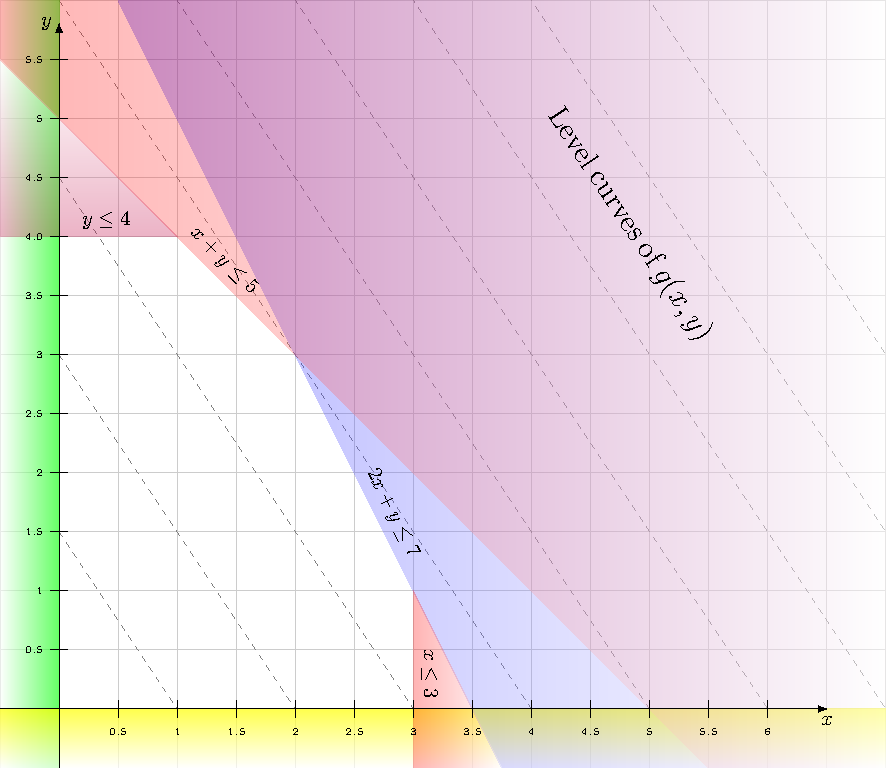
\includegraphics[width=0.6\textwidth]{figures/linear_algebra/linear_programming_feasible_region.pdf}
		% TODO: add x >0 and y >0 labels in bottom left corner 
		\end{center}
		\vspace{-6mm}
		\caption{The \emph{feasible region} for the linear programming problem. 
				The feasible region is the subset of the $xy$-plane that contains points $(x,y)$ satisfying all the constraints.
				}
		\label{fig:linear_programming_feasible_region}
		\end{figure}

	\noindent
	\textbf{Which feasible point produces the maximum value of $g(x,y)$?}
	This is the question we aim to answer in linear programming.
	%
	The linear programming problem illustrated in Figure~\ref{fig:linear_programming_feasible_region} is
	simple enough that you can solve it by simply looking at the graph.
	The highest level curve that touches the feasible region is $g(x,y)=12\,000$,
	and the feasible point that lies on this level curve is $(2,3)$.
	The solution to the optimization problem is:
	\[
		\max_{(x,y) \textrm{ feasible}} g(x,y) = 12\,000
		\qquad
		\textrm{and}
		\qquad
		\mathop{\textrm{argmax}}_{(x,y) \textrm{ feasible}} g(x,y) = (2,3).
	\]
	%
	Real-life linear programming problems usually involve hundreds of variables,
	so it's not possible simply to ``look'' at the constraint region and find the optimal solution.
	%	---unless you can see surfaces and inequalities in 100-dimensions.
	%	Wow how much coffee did you drink to do that?
	We need to develop a systematic approach---an algorithm---which doesn't
	depend on our ability to visualize the geometry of high-dimensional surfaces.
		
	
\subsection{Simplex algorithm}
\label{applications:simplex_algorithm}
	
	
	The \emph{simplex algorithm}, invented in 1947, 
	is a systematic procedure for finding optimal solutions to linear programming problems.	
	The main idea of the simplex algorithm is to start from one of the corner points of the 
	feasible region and ``move'' along the sides of the feasible region until we find the maximum.
	The reason why this ``sticking to the sides'' strategy works is that maximum solutions to linear programming
	problems always occur at the corners of the feasible region.
	Therefore, we're sure to find the maximum if we visit all the corners.
	Furthermore, in each iteration of the simplex algorithm we will always move along an edge where $g(x,y)$ increases.
	Thus by moving from edge to edge in directions where $g(x,y)$ increases,
	sooner or later we'll reach the corner point where $g(x,y)$ is maximum.
	
	The steps of the simplex algorithm are as follows:
	
	\begin{description}[style=unboxed]
	\item[INPUTS:] Objective function $g(\vec{x})$ and constraints of the form $\vec{a}_i \cdot \vec{x} \leq b_i$.
	\item[SETUP:] Construct the \emph{tableau}:
		\begin{itemize}
			\item Place constraint equations and slack variables in the first rows.
			\item Place $-g(\vec{x})$ in the last row of the tableau.
		\end{itemize}
	\item[INITIALIZATION:]  Start the algorithm from the coordinates $\vec{x}_0$ that correspond 
		to a vertex of the constraint region.
	\item[MAIN LOOP:] Repeat while negative numbers in the last row of the tableau exist: 
		\begin{description}[style=unboxed]
			\item[Choose pivot variable:] The pivot variable is the most negative number in the last row of the tableau. 
			\item[Choose pivot row:] The pivot row corresponds to the first constraint that will become active when the pivot variable increases.
			\item[Move:] The algorithm ``moves'' from the vertex with coordinates $\vec{x}$ to the vertex with coordinates $\vec{x}^\prime$,
					which is defined as a vertex where the pivot row is active.
			\item[Change of variables:]	
				 Perform the change of variables from the coordinates system $B$ with origin at $\vec{x}$ 
				 to a coordinates system $B^\prime$ with origin at $\vec{x}^\prime$.
				 This involves row operations on the tableau.
		\end{description}
	\item[OUTPUT:] When no more negative numbers in the last row exist, 
		we have reached an optimal solution $\vec{x}^* \equiv \mathop{\textrm{argmax}}_{\vec{x}} g(\vec{x})$.
	
	\end{description}
	
	
	\noindent
	Though not exactly identical to the Gauss--Jordan elimination procedure,
	the simplex algorithm is similar to it because it depends on the use of row operations.
	For this reason, linear programming and the simplex algorithm are often inflicted upon 
	students taking a linear algebra course, especially business students.	
	I'm not going to lie to you and tell you the simplex algorithm is simple,
	but it is very powerful so you should know it exists, 
	and develop a general intuition about how it works.
	Like with all things corporate-related,
	it's worth learning about them so you'll know the techniques of the enemy.

	In the remainder of this section, we'll go through the steps of the simplex algorithm 
	needed to find the optimal solution to the Xapper-and-Yapper production problem.
	We'll analyze the problem from three different angles: 
	graphically by drawing shifted coordinate systems,
	analytically by writing systems of equations, 
	and computationally by using a new matrix-like structure called a \emph{tableau}.
	%which is useful for performing simplex algorithm calculations.
	%
	
	
	\subsubsection{Definitions}
		
		We now introduce some useful terminology used in linear programming:
		
		\begin{itemize}
			\item An inequality $a_1x+a_2y \leq b$ is \emph{loose} (or \emph{slack}) for a given $(x,y)$ 
				if there exists a positive constant $s >0$ such that $a_1x+a_2y +s = b$. 
			\item An inequality $a_1x+a_2y \leq b$ is \emph{tight} for a given $(x,y)$ if the equality conditions holds $a_1x+a_2y = b$.
			\item  $s$: \emph{slack variable}. Slack variables can be added to any inequality $a_1x+a_2y \leq b$ 
				to transform it into an equality $a_1x+a_2y +s =b$. Note slack variables are always nonnegative $s \geq 0$.
			\item A \emph{vertex}   of an $n$-dimensional constraint region is a point where $n$ inequalities are tight.

			\item An \emph{edge} of an $n$-dimensional constraint region is place where $n-1$ inequalities are tight.
			\item	A \emph{pivot variable} is a variable whose increase leads to an increase in the objective function.
			\item	A \emph{pivot row} is a row in the tableau that corresponds to the currently active edge during 
				a ``move'' operation of the simplex algorithm.
			\item $\vec{v}$: a vector that represents the current \emph{state} of the linear program.
			\item A \emph{tableau} is a matrix that represent the constraints on the feasible region 
				and the current value of the objective function.
				Tableaus allow us to solve linear programming problems using row operations.
		\end{itemize}
	
	
	\subsubsection{Introducing slack variables}
	
		In each step of the simplex algorithm,
		we'll keep track of which constraints are \emph{active} (tight) and which are \emph{inactive} (loose).
		%
		To help with this bookkeeping task,
		we introduce nonnegative a \emph{slack variable} $s_i \geq 0$ for each of the inequality constraints.
		%
		If $s_i > 0$, inequality $i$ is loose (not active),
		and if $s_i=0$, inequality $i$ is tight (active).
		If we want to remain within the feasible region, 
		no $s_i$ can become negative, 
		since $s_i< 0$ implies inequality $i$ is not satisfied.
		
		Introducing the slack variables, the linear program becomes:
		\begin{align*}
			\qquad \qquad   \max_{x,y} 	g(x,y) &= 3000x + 2000y, 	\\  
		\intertext{subject to the equality constraints:}
					x 	\ \ \quad	+s_1 \quad \quad \quad	\ &=	\ 3,	\\
						y       \quad +s_2 \quad \quad   		\ &= 	\ 4,	\\
					2x	+ y	\quad \quad + s_3 \quad 		\ &= 	\ 7,	\\
					x 	+ y	\quad \quad \quad + s_4  		\ &= 	\ 5,	\\
						x,y,s_1,s_2,s_3,s_4				\ &\geq \	0. \\
		\end{align*}	
		
		\noindent
		This is starting to look a lot like a system of linear equations, right?
		Recall that what matters the most in systems of linear equations are the \emph{coefficients},
		and not the variable names. 
		Previously, 
		when faced with overwhelming complexity in the form of linear equations with many variables, 
		we used an augmented matrix to help us focus only on what matters.
		We'll use a similar approach again.


	\subsubsection{Introducing the tableau}

		A \emph{tableau} is a compact representation of a linear programming problem in the form of an array of numbers, 
		analogous to the augmented matrix used to solve systems of linear equations.
		{\footnotesize
		\[
			\begin{array}{rl}
					x \ \ \quad	+s_1 \quad \quad \quad		\ &=	\ 3	\\
						y       \quad +s_2 \quad \quad   		\ &= 	\ 4	\\
					2x	+ y	 \quad \quad + s_3 \quad		\ &= 	\ 7	\\
					x 	+ y	\quad \quad \quad + s_4  		\ &= 	\ 5	\\
		        - 3000x  -   2000y   \quad \quad \ \ \, 	\	\ &= \ \underline{?}
			\end{array} 
			\quad
			\Leftrightarrow
			\quad
			\left[
			\begin{array}{rrrrrr|r}
				    1&     0& 1& 0& 0& 0 \ \ & \ 3     \\ 
				    0&     1& 0& 1& 0& 0 \ \ & \  4     \\ 
				    2&     1& 0& 0& 1& 0 \ \ & \  7     \\ 
				    1&     1& 0& 0& 0& 1\ \ & \  5    \\ 
				\!\!\!-3000& \!\!\!\!-2000& 0& 0& 0& 0 \ \ & \  \underline{?}
			\end{array}
			\right]\!.
		\]}%
		
		\noindent
		The first six columns of the tableau correspond to the variables $x$, $y$, $s_1$, $s_2$, $s_3$, $s_4$,
		and the last column contains the constants from the constraint equations.
		%
 		In the last row, we use the coefficients of the negative objective function $-g(x,y)$.
		This strange initialization of the last row of the tableau is a trick we use to calculate the current value of the objective function $g(x,y)$
		in the bottom right corner of the tableau (the entry that contains an underlined question mark in the above tableau).
		We defer the explanation of why we use the \emph{negative} of the objective function 
		in the last row until after we learn about the interpretation of row operations on the tableau.
		
		The numbers in the example problem are deliberately chosen to emphasize the distinction between
		the constraint rows and the objective-function row.
		Small coefficients are used for the constraints and large coefficients in the objective function.
		%		(the sides of the region)  vs level curves
		This way it should be clear that two different types of data are recorded in the tableau.
		%

		Looking back to Figure~\ref{fig:linear_programming_feasible_region}
		can help you compare the two scales of the problem: 
		the linear constraints that delimit the feasible region all fit in a $6\times 6$ coordinate system,
		while the distance between the level curves of $g(x,y)$ is $3000$.
		%
		You can think of the linear programming problem described in Figure~\ref{fig:linear_programming_feasible_region}
		as a three dimensional plot of the plane $z=g(x,y)=3000x+2000y$,
		restricted to the points that lie above the feasible region.
		%
		The scale of the $x$- and $y$-axes in such a plot would be much smaller than the scale of the $z$-axis.
		% TODO: produce 3d plot of constraint region.
		
		

	\subsubsection{Start from a vertex}
	
		In each step of the simplex algorithm,
		we want to move from one vertex of the constrain region to another vertex,
		moving along one of the sides.
		%
		For the algorithm to do its thing,
		it must start from one of the corners of the constraint region.
		%
		We can start from the origin $(0,0)$,
		which is the vertex formed by the intersection of the nonnegativity constraints $x\geq 0$, and $y \geq 0$.
		
		Given $x=0$ and $y=0$, we can deduce the values of the slack variables: 
		$s_1=3$, $s_2=4$, $s_3=7$, $s_4=5$.
		In other words, all constraints are initially maximally slack.
		
	\subsubsection{State vector}

		The simplex algorithm requires two types of state.
		First, we must record the coordinates $(x,y)$ of the current position (the current vertex being visited).
		Second, we need to keep track which constraints are tight and which are slack.
		
		Now this is where things get a little weird.
		Instead of keeping track of these two types of information separately,
		we'll use a six-dimensional \emph{state vector} that represents the current position \emph{in terms of} the variables in the tableau.
		%
		The state vector that corresponds to starting the simplex algorithm from $(x,y)=(0,0)$ is
		\[
		   \vec{v} = (0,0, 1, 1, 1, 1 ).
		\]
		If the $i$\textsuperscript{th} entry of $\vec{v}$ is $1$ then the $i$\textsuperscript{th} column of the tableau is used in the current set of equations.
		Otherwise if the $i$\textsuperscript{th} entry of $\vec{v}$ is $0$ then the $i$\textsuperscript{th} column of the tableau
		should be ignored.\!\footnote{Readers familiar with programming will recognize $\vec{v}$ serves as a \emph{bitmask}.}
		
		Note that each state vector is tied to a particular tableau and has no meaning on its own.
		%
		We can understand the select-only-columns-with-one-in-the-state procedure as a matrix multiplication:
		{\footnotesize
		\[
			\left[
			\begin{array}{rrrrrr}
				    1&     0& 1& 0& 0& 0      \\ 
				    0&     1& 0& 1& 0& 0       \\ 
				    2&     1& 0& 0& 1& 0       \\ 
				    1&     1& 0& 0& 0& 1        \\ 
				\!\!\!-3000& \!\!\!\!-2000& 0& 0& 0& 0  
			\end{array}
			\right]	
			\!\!
			\begin{bmatrix}
				0 \\ 0 \\  1 \\ 1 \\ 1 \\ 1 
			\end{bmatrix}\!
			=
			\!
			\begin{bmatrix}
				3 \\ 4 \\  7 \\ 5 \\ 0 
			\end{bmatrix}			
			\quad	
			\Rightarrow
			\ \ \
			\begin{array}{rl}
					s_1 \quad \quad \quad		\ &=	 3	\\
					\quad s_2 \quad \quad 		\ &= 	 4	\\
					\quad \quad  s_3 \quad 		\ &= 	 7	\\
					 \quad \quad \quad  s_4   		\ &= 	 5	\\
			        - 3000(0)  -   2000(0)     \!\!&=  0.
			\end{array} 				
		\]}%
		The current problem variables have value $x=0$ and $y=0$,
		and each of the constraint equations is maximally slack.
		The value of the objective function at this vertex is $g(0,0)=0$.
		
		I know what you're thinking.
		Surely it would have been simpler to keep track of the position $(x,y)$ 
		and the slackness separately $(s_1,s_2,s_3,s_4)$,
		rather than to invent a binary state vector $\vec{v} \in \{0, 1\}^{6}$,
		and then depend on matrix multiplication to find the coordinates.
		%
%		and thus operate on them simultaneously through row operations.
		%	You'll see things will become clear when we start with the row operations,
		%	but before we move on let's just look at Figure~\ref{fig:linear_programming_1} to see where we are.
		
		True that. 
		But the energy we invested to represent the constraints as a tableau 
		will allow us to perform complex geometrical operations by performing row operations on the tableau.
		%
		The key benefit of the combined representation is that it treats 
		problem variables and slack variables on the same footing.
		
		\begin{figure}[htb]
		\begin{center}
		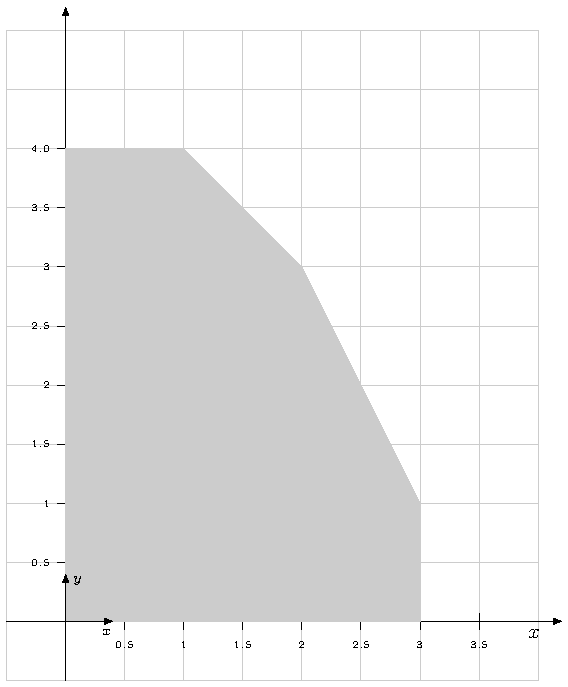
\includegraphics[width=0.5\textwidth]{figures/linear_algebra/linear_programming_1.pdf}
		\end{center}
		\vspace{-6mm}
		\caption{The $(x,y)$ coordinates are measured with respect to $(0,0)$.}
		\label{fig:linear_programming_1}
		\end{figure}


		
		It's now time to start making progress. 
		Let's make a move. Let's cut some slack!

		
		
	\subsubsection{Choose the pivot variable}

		The simplex algorithm continues while there exist negative numbers in the last row of the tableau.
		Recall we initialized the last row of the tableau with the coefficients of $-g(x,y)$
		and the initial value to $g(0,0)=0$.
		%
		\[
			\left[
			\begin{array}{rrrrrr|r}
				    1&     0& 1& 0& 0& 0 \ \ & \ 3    \  \   \\ 
				    0&     1& 0& 1& 0& 0 \ \ & \  4    \  \   \\ 
				    2&     1& 0& 0& 1& 0 \ \ & \  7    \  \   \\ 
				    1&     1& 0& 0& 0& 1\ \ & \  5      \  \ \\ 
				-3000& -2000& 0& 0& 0& 0 \ \ & \  0      \  \ 
			\end{array}
			\right].
		\]
		Both the $x$ and $y$ columns contain negative numbers.
		This means the objective function would increase if were to increase either the $x$ or the $y$ variables.
		%
		The coefficient $-3000$ in the last row represents our \emph{incentives} towards increasing the variable $x$:
		each increase of $1$ step in the Xapper production will result 	in an increase of $3000$ in the value of $g(x,y)$.
		Similarly, the coefficient $-2000$ indicates that a unit-step in the $y$ direction will increase $g(x,y)$ by $2000$.
		It's a bit complicated why we put the \emph{negatives} of the coefficients in the row for the objective function,
		but you'll have a chance to convince yourself it all works out nicely when you see the row operations.

		Given the options $x$ and $y$,
		we choose to increase the $x$ variable since it leads to a biggest gain in profits.
		Remember, we're playing the role of the greedy corporate capitalist whose only motivation is to maximize profits.
		
		
	\subsubsection{Choose the pivot row}
	
		We've decided to increase the $x$ variable.
		The next step is to check how big we can make the $x$ variable before hitting one of the constraints.
		%
		% To find out we check each of the four constraints to find which will become active 
		%		We say $x$ is the \emph{pivot variable}---the variable 
		
		Which constraint do we hit first when we move in the $x$ direction?
		In the first equation $x + s_1 = 3$, we could increase $x$ up to $x=3$.
		In the second equation $y + s_2 = 0 + s_2 = 4$, the $x$-variable doesn't appear so it ``allows'' an arbitrary increase in $x$.
		The third constraint $2x + y + s_3 = 2x + 0 + s_3  = 7$ allows an increase in $x$ up to $x \leq 7/2=3.5$.
		Finally, the fourth equation  $x + 0+ s_4 = 5$ imposes the constraint $x\leq 5$.		

		The equation $x + s_1 = 3$ allows the smallest increase in $x$,
		so this equation will become our \emph{pivot row}.
		Specifically, pivoting through the equation $x + s_1 = 3$ means we're decreasing $s_1$ from $3$ to $0$ 
		and correspondingly increasing $x$ from $0$ to $3$.
		We have thue de-slacked the constraint $x + s_1 = 3$.
		
		Performing the pivot operation corresponds to the following change in the state vector:
		\[
		   \vec{v} = (0,0, 1, 1, 1, 1 )
		   \qquad  \to 
		   \qquad 
		   \vec{v}^{\prime} = (1,0, 0, 1, 1, 1 ).
		\]
		To understand the effect of this change of state,
		let's look at the constraint equations that result from the new state vector:
		{\footnotesize
		\[
			\left[
			\begin{array}{rrrrrr}
				    1&     0& 1& 0& 0& 0     \  \   \\ 
				    0&     1& 0& 1& 0& 0     \  \   \\ 
				    2&     1& 0& 0& 1& 0     \  \   \\ 
				    1&     1& 0& 0& 0& 1       \  \ 
					%				    \\ 
					%				-3000& -2000& 0& 0& 0& 0       \  \ 
			\end{array}
			\right]	
			\!\!
			\begin{bmatrix}
				1 \\ 0 \\  0 \\ 1 \\ 1 \\ 1 
			\end{bmatrix}
			=
			\begin{bmatrix}
				3 \\ 4 \\  7 \\ 5 \\ 0 
			\end{bmatrix}			
			\qquad	
			\Rightarrow
			\qquad
			\begin{array}{rl}
					x \ + \ \ \  \quad \quad \quad	\ &=	\ 3	\\
					\quad s_2 \quad \quad 		\ &= 	\ 4	\\
					\quad \quad  s_3 \quad 		\ &= 	\ 7	\\
					 \quad \quad \quad  s_4   		\ &= 	\ 5 \ .
			%			        - 3000(0)  -   2000(0)      \quad \  &= \ \underline{0}
			\end{array}
		\]}%
		The effect of the new state $\vec{v}^\prime$ is to increase $x$ from $0$ to $3$,
		which leads to corresponding decrease of $s_1$ from $3$ to $0$.
		The value of the six variables are now:
		\[
			x=3, \quad y=0, \quad s_1=0, \quad s_2=4,  \quad s_3=7, \quad s_4=5.
		\]
		%
		Note the change of state vector $\vec{v} \to \vec{v}^\prime$ we performed did not change the 
		system of equations that describe the constraints of the linear program:
		\[		
			\begin{array}{rl}
					x \ + \ \ \ \ \ + \ s_1 \quad \quad \quad	\ &=	\ 3	\\
					          y \ + \quad s_2 \quad \quad 		\ &= 	\ 4	\\
					2x \ + \ y \ + \quad \quad  s_3 \quad 		\ &= 	\ 7	\\
					 \ x \ + \ y \ + \quad \quad \quad  s_4   		\ &= 	\ 5.	
			\end{array}
		\]			
		%
		This system of equations corresponds to the tableau:
		\[
			\left[
			\begin{array}{rrrrrr|r}
				    1&     0& 1& 0& 0& 0 \ \ & \ 3    \  \   \\ 
				    0&     1& 0& 1& 0& 0 \ \ & \  4    \  \   \\ 
				    2&     1& 0& 0& 1& 0 \ \ & \  7    \  \   \\ 
				    1&     1& 0& 0& 0& 1\ \ & \  5      \  \ \\ 
				-3000& -2000& 0& 0& 0& 0 \ \ & \  0      \  \ 
			\end{array}
			\right].
		\]
		Except for the increase in $x$ and the corresponding decrease in $s_1$,
		we haven't done anything to the tableau.
		The next step of the simplex algorithm involves performing row operations on the tableau.
		
	\subsubsection{Change of variables}
		
		Knowing $x=3$, we can subtract this equation from the other constraints,
		to remove the variable $x$ from the system of equations.
		We can eliminate the variable $x$ from the system of equations 
		by performing the following row operations:
		\begin{itemize}
			\item $R_3 \gets R_3 - 2R_1$
			\item $R_4 \gets R_4 - R_1$
			\item $R_5 \gets R_5 + 3000R_1$
		\end{itemize}
		%		>>> M.row(2& lambda v,j: v-2*M[0,j] )
		%		>>> M.row(3& lambda v,j: v-1*M[0,j] )
		%		>>> M.row(4& lambda v,j: v+3000*M[0,j] )
		
		\noindent
		The result is the following tableau:
		\[
			\left[
			\begin{array}{rrrrrr|r}
		1&     0&    1& 0& 0& 0&    3      \\ 
		0&     1&    0& 1& 0& 0&    4      \\ 
		0&     1&   -2& 0& 1& 0&    1      \\ 
		0&     1&   -1& 0& 0& 1&    2      \\ 
		0& -2000& 3000& 0& 0& 0& 9000      
			\end{array}
			\right].
		\]
		Geometrically speaking,
		the effect of the row operations is a change of coordinate system.
		The equations in the new tableau are expressed with respect to the 
		coordinate system $(x',y')$ whose origin is at $(3,0)$.
		Figure~\ref{fig:linear_programming_1} illustrates this change of coordinate system:
		
		\begin{figure}[htb]
		\begin{center}
		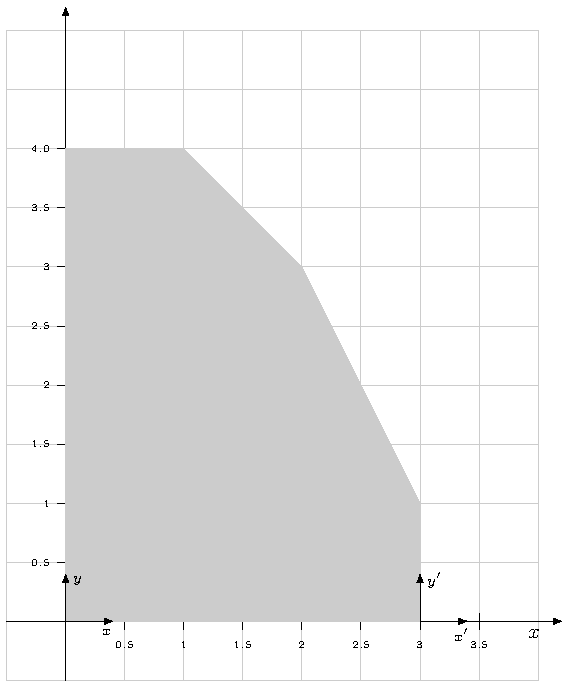
\includegraphics[width=0.5\textwidth]{figures/linear_algebra/linear_programming_2.pdf}
		\end{center}
		\vspace{-6mm}
		\caption{The origin of the original $(x,y)$ coordinates system is at $(0,0)$. 
				The origin of the new $(x',y')$ coordinates system is at $(3,0)$.}
		\label{fig:linear_programming_1}
		\end{figure}


		The values of the six variables after performing the change of coordinate system are:
		\[
			x=3, \quad y'=0, \quad s'_1=0, \quad s'_2=4,  \quad s'_3=1, \quad s'_4=2,
		\]		
		and the current state of the tableau is 
		\vspace{1mm}
		{\footnotesize
		\[		
			\left[
			\begin{array}{rrrrrr|r}
				1&     0&    1& 0& 0& 0&    3      \\ 
				0&     1&    0& 1& 0& 0&    4      \\ 
				0&     1&   -2& 0& 1& 0&    1      \\ 
				0&     1&   -1& 0& 0& 1&    2      \\ 
				0& -2000& 3000& 0& 0& 0& 9000      
			\end{array}
			\right]			
			\quad
			\Leftrightarrow
			\quad		
			\begin{array}{rl}
				x \ + \ \ \ \ \ + \, \ \  s'_1 \quad \quad \quad	\ &=	\ 3	\\
				          y' \ + \quad \ \  s'_2 \quad \quad 		\ &= 	\ 4	\\
				 y' \ - \ 2s'_1 \quad  s'_3 \quad 		\ &= 	\ 1	\\
				 y' \ - \, \ \ s'_1 \quad \quad  s'_4   		\ &= 	\ 2.
			\end{array} 				
		\]}%		
		Note $s'_1=0$ in the system of equations so we could completely ignore this variable and the associated column of the tableau.
		Nevertheless,  we choose to keep the $s'_1$ column around as a bookkeeping device,
		because it's useful to keep track of how many times we have subtracted the first row from the other rows.

		We have now completed the first step in of the simplex algorithm,
		and we continue the procedure by looking for the next pivot.
		
		
	\subsubsection{Choose the pivot}
	
		Observe the second column of the row that corresponds to the objective function contains a negative number,
		which means the objective function will increase if we increase the variable $y$.
		% advantageous

		
		Having decided to increase $y'$ we must now 
		By what amount can we increase variable $y'$ before we hit one of the constraints?
		We can find out by computing the ratios of the constants in the rightmost column of the tableau,
		and the $y'$ coefficients of each row.
		The first constraint does not contain $y'$ at all, so it allows any increase in $y'$.
		The second constraint will become active when $y' = 4$.
		The third constraint allows $y'$ to go up to $y'=1$,
		and the fourth constraint becomes active when $y'=2$.
		%>>> [  M[i,6]/M[i,1] for i in range(0,4) ]
		%[oo& 4& 1& 2]
		%
		The largest increase in $y'$ we can make is $y'=1$.
		We will use the third row of the tableau as the \emph{pivot row},
		which means we de-slack $s'_3$ from $1$ to $0$ and correspondingly increasing $y'$ from $0$ to $1$.
		After pivoting, the values of the six variables are
		\[
			x'=3, \quad y'=1, \quad s''_1=0, \quad s''_2=4,  \quad s''_3=0, \quad s''_4=2.
		\]
		
		
	\subsubsection{Change of variables}
	
		We can now subtract the equation $y'=1$ from the other $y'$-containing rows.
		The required row operations are
		\begin{itemize}
			\item $R_2 \gets R_2 - R_3$
			\item $R_4 \gets R_4 - R_3$
			\item $R_5 \gets R_5 + 2000R_3$
		\end{itemize}		
		%>>> M.row(1& lambda v,j: v-1*M[2,j] )
		%>>> M.row(3& lambda v,j: v-1*M[2,j] )
		%>>> M.row(4& lambda v,j: v+2000*M[2,j] )
		After applying these row operations, the resulting tableau is
		\[
		\left[
		\begin{array}{rrrrrr|r}
		1& 0&     1& 0&    0& 0&     3      \\ 
		0& 0&     2& 1&   -1& 0&     3      \\ 
		0& 1&    -2& 0&    1& 0&     1      \\ 
		0& 0&     1& 0&   -1& 1&     1      \\ 
		0& 0& -1000& 0& 2000& 0& 11000      
		\end{array}
		\right].		
		\]
		
		\noindent
		The geometrical interpretation of subtracting the equation $y'=1$ from the other constraints
		is a change to a new coordinate system $(x'',y'')$ with origin at $(3,1)$,
		as illustrated in Figure~\ref{fig:linear_programming_3}.
		
		\begin{figure}[htb]
		\begin{center}
		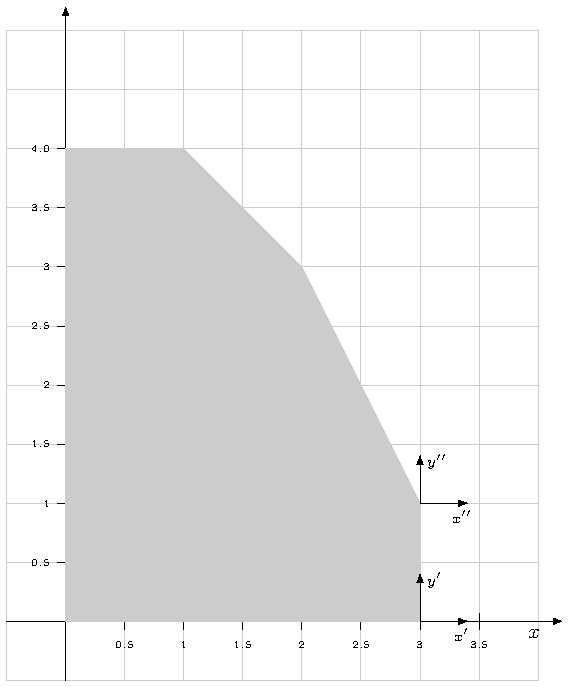
\includegraphics[width=0.5\textwidth]{figures/linear_algebra/linear_programming_3.pdf}
		\end{center}
		\vspace{-6mm}
		\caption{The origin of the $(x'',y'')$ coordinate system is at $(3,1)$.}
		\label{fig:linear_programming_3}
		\end{figure}

		

	\subsubsection{Choose a pivot}
	
		The third column of the tableau contains a negative number,
		which means the objective function will increase if we increase $s''_1$.
		We pick $s''_1$ as the next pivot variable.
		
		We now check the different constraints containing $s''_1$ to see which will become
		active first when we increase $s''_1$.
		The first inequality imposes $s''_1 \leq 3$,
		the second imposes $s''_1 \leq 3/2=1.5$,
		the third equation contains a negative amount of $s''_1$ and thus can't be used as a pivot.
		The equation in the fourth row, $s''_1 -s''_3 + s'_4 = 1$,
		imposes the constraint $s''_1 \leq 1$,
		and is the tightest constraint.
		Therefore, we'll use the fourth row equation as the pivot.
		%>>> [  M[i,6]/M[i,2] for i in range(0,4) ]
		%[3& 3/2& -1/2& 1]
		
		After pivoting, the new values of the variables are
		\[
			x''=3, \quad y''=1, \quad s''_1=1, \quad s''_2=4,  \quad s''_3=0, \quad s''_4=0.
		\]
		We now carry out the following row operations to eliminate $s''_1$ from the other eqations:
		\begin{itemize}
			\item $R_1 \gets R_1 - R_4$
			\item $R_2 \gets R_2 - 2R_4$
			\item $R_3 \gets R_3 + 2R_4$
			\item $R_5 \gets R_5 + 1000R_4$
		\end{itemize}				
		%>>> M.row(0& lambda v,j: v-1*M[3,j] )
		%>>> M.row(1& lambda v,j: v-2*M[3,j] )
		%>>> M.row(2& lambda v,j: v+2*M[3,j] )
		%>>> M.row(4& lambda v,j: v+1000*M[3,j] )		

		\noindent
		The final tableau is
		\[
		\left[
		\begin{array}{rrrrrr|r}
		1& 0& 0& 0&    1&   -1&     2      \\ 
		0& 0& 0& 1&    1&   -2&     1      \\ 
		0& 1& 0& 0&   -1&    2&     3      \\ 
		0& 0& 1& 0&   -1&    1&     1      \\ 
		0& 0& 0& 0& 1000& 1000& 12000      
		\end{array}
		\right].
		\]
		We state variables that correspond to this tableau are
		\[
			x'''=2, \quad y'''=3, \quad s'''_1=1, \quad s'''_2=1,  \quad s'''_3=0, \quad s'''_4=0.
		\]	
		We know this tableau is \emph{final} because there are no more negative numbers in the last row.
		This means there are no more directions we can move in that would increase the objective function.
		%

		\begin{figure}[htb]
		\begin{center}
		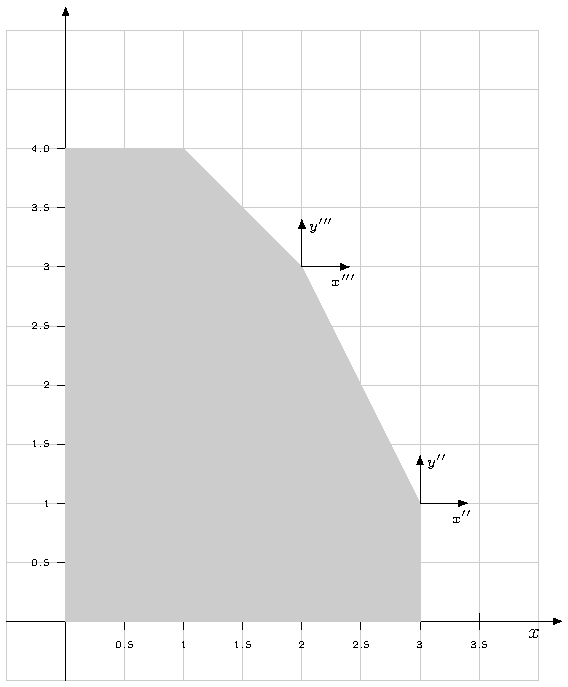
\includegraphics[width=0.5\textwidth]{figures/linear_algebra/linear_programming_4.pdf}
		\end{center}
		\vspace{-3mm}
		\caption{The $(x''',y''')$ coordinates are measured with respect to the point $(2,3)$. 
				The simplex algorithm stops because it's not possible to increase any variable 
				in a direction to increase the objective function $g(x,y)$.}
		\label{fig:linear_programming_4}
		\end{figure}
		


	\subsubsection{Regroup}

		If you're finding linear programming and the simplex algorithm difficult to comprehend,
		you're not alone. 
		It will take some time to understand the procedure,
		but if you solve a few practice problems, you'll get the hang of it.
			
		Linear programming problems with few parameters and few constraints are simple to solve, 
		but problems that involve hundreds of variables and hundreds of constraints can be very difficult solve.
		Linear programming problems with hundreds and even thousands of variables are common in real-world scenarios.
		For this reason, it is very important to approach linear programming problems 
		in a systematic manner so that we can teach a computer to do the steps for us.
		In the next section we enlist the help \texttt{SymPy} to retrace the steps of the simplex algorithm for the Xapper--Yapper linear program.
				

\subsection{Using \texttt{SymPy} to solve linear programming problems}

	Recall each \texttt{SymPy} \texttt{Matrix} object has a method called \texttt{.row(...)} that
	can be used to perform row operations on the matrix.
	%
	Let's see if we can't make linear programming a little bit more bearable by using \texttt{SymPy}
	to perform the row operations on the tableau.
	Letting \texttt{SymPy} do the tedious row operations work for us will 
	let us focus on the \emph{state} of the algorithm in each step.
	
	Since \texttt{SymPy} will be doing the calculations for us,
	it will not hurt if we include the nonnegativity constraints $x\geq0$ and $y\geq 0$ into our analysis.
	%		See Figure~\ref{fig:linear_programming_feasible_region} (page~\pageref{fig:linear_programming_feasible_region})
	%		for an illustration of the constraint region.
	We rewrite these constraints as $-x \leq 0$ and $-y \leq 0$ in order to conform to the standard convention ($a_1x+a_2y \leq b$) 
	for expressing constraints.

	The full system of constrains that correspond to the feasible region is
	\[
		\begin{array}{rl}
				x \ \ \quad	+s_1 \quad \quad \quad \quad \quad		\ &=	\ 3	\\
					y       \quad +s_2 \quad \quad \quad \quad 		\ &= 	\ 4	\\
				2x	+ y	 \quad \quad + s_3 \quad \quad \quad		\ &= 	\ 7	\\
				x 	+ y	 \quad \quad \quad + s_4 \quad \quad 		\ &= 	\ 5	\\
				-x \ \ \	 	\quad \ \ \quad \quad \quad +s_5 \quad 		\ &=	\ 0	\\
					-y       \quad \quad \quad \quad \quad + s_6   		\ &= 	\ 0.	\\
		\end{array} 		
	\]
	
	\noindent
	We can create a tableau as a \texttt{SymPy} matrix object whose coefficients 
	correspond to the above system of equations. Use the following command:
\begin{verbatim}
>>> M = Matrix([
[    1,    0,  1, 0, 0, 0, 0, 0, 3]
[    0,    1,  0, 1, 0, 0, 0, 0, 4]
[    2,    1,  0, 0, 1, 0, 0, 0, 7]
[    1,    1,  0, 0, 0, 1, 0, 0, 5]
[   -1,    0,  0, 0, 0, 0, 1, 0, 0]
[    0,   -1,  0, 0, 0, 0, 0, 1, 0]
[-3000,-2000,  0, 0, 0, 0, 0, 0, 0]] )
\end{verbatim}

	\noindent
	Note  constructing the tableau did not require any special command---a tableau is just a regular \texttt{Matrix} object.
	The first six rows of the matrix~$M$ correspond to the constraints on the feasible region,
	while the last row contains the negatives of the coefficients of the objective function $-g(x,y)=-3000x-2000y$.
	

	\subsubsection{Vertices and sides}
	
		The simplex algorithm starts from a \emph{vertex} of the feasible region,
		and moves along the \emph{edges} of the feasible region.
		For the two-dimensional Xapper--Yapper production problem,
		the vertices of the region are the corners,
		and the edges are the sides of a two-dimensional \emph{polygon}.
		A polygon is the general math term for describing a subset of the $xy$-plane
		delimited by a finite chain of straight line segments.
		
		More generally,
		the constraint region of an $n$-dimensional linear programming problem has the shape of an $n$-dimensional \emph{polytope}.
		A vertex of the polytope corresponds to a place where $n$ constraint inequalities are satisfied,
		while an edge corresponds to the intersection of $n-1$ inequalities.		
		In each step of the simplex algorithm,
		we'll keep track of which constraints in the tableau are \emph{active} (tight) and which are \emph{inactive} (loose).
		
		The simplex algorithm must be started from one of the vertices of the rate region.
		For the Xapper--Yapper production problem,
		we initialized the tableau from the corner $(0,0)$,
		which is the vertex where the two nonnegativity constraints intersect.
				
\begin{verbatim}
>>> M
[    1,     0, 1, 0, 0, 0, 0, 0, 3]
[    0,     1, 0, 1, 0, 0, 0, 0, 4]
[    2,     1, 0, 0, 1, 0, 0, 0, 7]
[    1,     1, 0, 0, 0, 1, 0, 0, 5]
[   -1,     0, 0, 0, 0, 0, 1, 0, 0]  (active)
[    0,    -1, 0, 0, 0, 0, 0, 1, 0]  (active)
[-3000, -2000, 0, 0, 0, 0, 0, 0, 0]
\end{verbatim}

		\noindent
		The current \emph{state} of the simplex algorithm is completely specified by the two \texttt{(active)} flags.
		We can deduce the value of all state variables from the knowledge that the inequalities
		$-x \leq  0$ and $-y \leq  0$ are tight.
		The fifth and sixths constraints are active,
		which means $s_5=0$ and $s_6=0$,
		from which we deduce that $x=0$ and $y=0$.
		If $x=0$ and $y=0$,
		then the other inequalities are maximally slack and thus $s_1=3$, $s_2=4$, $s_3=7$, $s_4=5$.
		

	\subsubsection{Choose the pivot 1}
	In the first step we choose to increase the $x$-variable since it leads to the bigger gain in $g(x,y)$
	($3000$ per unit step), 
	as compared to an increase in the $y$-direction ($2000$ per unit step).

	Next we must choose the pivot row.	
	How big of a step can we make in the $x$-direction before hitting some constraint?
	To calculate the maximum allowed step in each direction,
	you must divide the current slack available by the $x$ coefficient  in each inequality:
	
\begin{verbatim}
>>> [  M[i,8]/M[i,0] for i in range(0,4) ]
[3, oo, 7/2, 5]
\end{verbatim}

	\noindent
	The above magical python invocation computes the largest step in the $x$ direction allowed by constant in each constraint.
	Since the step size of the first row (index 0) is the smallest,
	we must choose the first row as our pivot.

	\subsubsection{Change of variables 1}
	Carry out the necessary row operations to eliminate all other numbers in the $x$ column.
	
\begin{verbatim}
>>> M.row(2, lambda v,j: v-2*M[0,j] )
>>> M.row(3, lambda v,j: v-1*M[0,j] )
>>> M.row(4, lambda v,j: v+1*M[0,j] )
>>> M.row(6, lambda v,j: v+3000*M[0,j] )
>>> M
[1,     0,    1, 0, 0, 0, 0, 0,    3]  (active)  
[0,     1,    0, 1, 0, 0, 0, 0,    4]
[0,     1,   -2, 0, 1, 0, 0, 0,    1]
[0,     1,   -1, 0, 0, 1, 0, 0,    2]
[0,     0,    1, 0, 0, 0, 1, 0,    3]
[0,    -1,    0, 0, 0, 0, 0, 1,    0]  (active)
[0, -2000, 3000, 0, 0, 0, 0, 0, 9000]
\end{verbatim}

	\noindent
	Again, the state of the linear program can be deduced from the information about which constraints are currently active.
	Since the first constraint is active ($s_1=0$), 
	we know $x=3$ and sixth inequality hasn't changed so we still have $y=0$.


	\subsubsection{Choose the pivot 2}
	This time we see there are gains to be had if we increase the $y$-variable,
	so we check which constraint will become active first as we increase the $y$-variable.
	Note we \texttt{M[i,1]} corresponds to the second column of the \texttt{Matrix} object \texttt{M}
	because \texttt{Python} uses $0$-based indexing.
	
\begin{verbatim}
>>> [  M[i,8]/M[i,1] for i in range(0,4) ]
[oo, 4, 1, 2].
\end{verbatim}

	\noindent
	The third row (index \texttt{2}) is the corresponds to the constrain that allows the smallest step
	in the $y$-direction,  so we must use the third row as our pivot.
	
	\subsubsection{Change of variables 2}	
	The next step is business as usual: we use a set of row operations to eliminate all the 
	$y$-coefficients above and below the third row.
	
\begin{verbatim}
>>> M.row(1, lambda v,j: v-1*M[2,j] )
>>> M.row(3, lambda v,j: v-1*M[2,j] )
>>> M.row(5, lambda v,j: v+1*M[2,j] )
>>> M.row(6, lambda v,j: v+2000*M[2,j] )
>>> M
[1, 0,     1, 0,    0, 0, 0, 0,     3]  (active)
[0, 0,     2, 1,   -1, 0, 0, 0,     3]
[0, 1,    -2, 0,    1, 0, 0, 0,     1]  (active)
[0, 0,     1, 0,   -1, 1, 0, 0,     1]
[0, 0,     1, 0,    0, 0, 1, 0,     3]
[0, 0,    -2, 0,    1, 0, 0, 1,     1]
[0, 0, -1000, 0, 2000, 0, 0, 0, 11000]
\end{verbatim}

	\noindent
	The first and the third row have become the active constraints,
	which means $x= 3$ and $2x+y= 7$.
	The full state of the algorithm is
	\[
		x=3, \quad y=1, \quad s_1=0, \quad s_2=3,  \quad s_3=0, \quad s_4=1.
	\]	

	%	\noindent
	%	\texttt{TODO: check  $s_2=3$ ??}
	%	\ \\
	%	\ \\
	
	
	\bigskip
	
	\subsubsection{Choose the pivot 3}
	The simplex algorithm continues because there still exists a negative coefficient
	in the objective function row of the tableau.
	The coefficient \texttt{-1000} in the column that corresponds to $s_1$ tells us 
	we can improve the value of the objective function if we increase the value of the $s_1$ variable.
	Increasing $s_1$ from its current value $s_1=0$ means we're making the first inequality ($x\leq3$) slack.

	The fourth constraint allows the smallest increase in the $s_1$-direction,
	as can be seen by the following calculation:	
\begin{verbatim}
>>> [  M[i,8]/M[i,2] for i in range(0,4) ]
[3, 3/2, -1/2, 1]
\end{verbatim}

	\noindent
	We choose the fourth row as our pivot.

	\subsubsection{Change of variables 3}	
	We can eliminate all the numbers in the $s_1$-column of the tableau
	using the following row operations:

\begin{verbatim}
>>> M.row(0, lambda v,j: v-1*M[3,j] )
>>> M.row(1, lambda v,j: v-2*M[3,j] )
>>> M.row(2, lambda v,j: v+2*M[3,j] )
>>> M.row(4, lambda v,j: v-M[3,j] )
>>> M.row(5, lambda v,j: v+2*M[3,j] )
>>> M.row(6, lambda v,j: v+1000*M[3,j] )
>>> M
[1, 0, 0, 0,    1,   -1, 0, 0,     2]
[0, 0, 0, 1,    1,   -2, 0, 0,     1]
[0, 1, 0, 0,   -1,    2, 0, 0,     3]  (active)
[0, 0, 1, 0,   -1,    1, 0, 0,     1]  (active)
[0, 0, 0, 0,    1,   -1, 1, 0,     2]
[0, 0, 0, 0,   -1,    2, 0, 1,     3]
[0, 0, 0, 0, 1000, 1000, 0, 0, 12000]
\end{verbatim}

	\noindent
	The simplex algorithm now terminates,
	since there are no more negative numbers in the last row.
	%
	The final state of the algorithm is 
	\[
		x=2, \quad y=3, \quad s_1=1, \quad s_2=1,  \quad s_3=0, \quad s_4=0.
	\]	
	The value of the function at this vertex is $g(2,3)= \$12000$.
	





	
	\subsection{Using a linear program solver}

		Using the \texttt{Matrix} row operations provided by \texttt{SymPy} is certainly a fast 
		method to perform the steps of the simplex algorithm.
		But there is an even better approach:
		we could outsource the work of solving the linear program 
		completely to the computer by using the function \texttt{linprog}
		that comes with the \texttt{Python} package \texttt{scipy}.
		
		These functions are not available in the web interface at \texttt{live.sympy.org},
		so you'll need to install \href{https://www.python.org/downloads/}{\texttt{Python}} 
		and the packages \href{http://www.scipy.org/install.html}{\texttt{numpy}}
		and \href{http://www.scipy.org/install.html}{\texttt{scipy}} on your computer.
		Once this is done, solving the linear program is as simple as 
		setting up the problem description and calling the function \texttt{linprog}:
		
\begin{verbatim}
>>> from scipy.optimize import linprog   
>>> c = [-3000, -2000]          # coefficients of f(x) 
>>> A = [[  1,  0],             # coefficients of the constraints
         [  0,  1],
         [  2,  1],
         [  1,  1],
         [ -1,  0],
         [  0, -1]]
>>> b = [3, 4, 7, 5, 0, 0]      # constraint constants 

>>> linprog(c, A_ub=A, b_ub=b)  # find min of f(x) s.t. Ax <= b
 success: True
       x: [ 2,  3] 
     fun: -12000
   slack: [ 1,  1,  0,  0,  2,  3]
 message: Optimization terminated successfully.
     nit: 3
\end{verbatim}

		\noindent
		The function \texttt{linprog} solves the \emph{minimization} problem $\min f(\vec{x})$,
		subject to the constraints $A\vec{x} \leq \vec{b}$.
		The objective function $f(x)\equiv \vec{c} \cdot \vec{x}$ is specified in terms of its 
		vector of coefficients $\vec{c}$.
		%
		We can't use \texttt{linprog} directly since the linear program we're trying to solve is a 
		maximization problem $\max g(\vec{x})$.
		To work around this mismatch between what we want to do and what the function can do for us,
		we can multiply the objective function by a negative sign.
		Finding the maximum of $g(\vec{x})$ is equivalent to finding the minimum of $f(\vec{x}) \equiv -g(\vec{x})$,
		since $\max g(\vec{x}) = \min -g(\vec{x}) = \min f(\vec{x})$.
		This is the reason why we specified the coefficients of the objective function as $\vec{c} = (-3000, -2000)$.
		We must also keep in mind the ``adaptor'' negative sign when interpreting the result:
		the minimum value of $f(\vec{x})$ is $-12\,000$, which means the maximum value of $g(\vec{x})=12\,000$.
		
		For more information about other linear program options you can supply,
		run the command \texttt{help(linprog)} from the \texttt{Python} command prompt.
		The package \texttt{scipy} supplies a number of other useful optimization functions,
		for quadratic programming, and optimization of non-linear functions.
		It's good if you understand details of the simplex algorithm
		(especially if you'll be asked to solve linear programs by hand on your exam),
		but make sure also know how to check your answers using the computer.
		
		Another useful computer tool is Stefan Waner's linear program solver,
		which can be accessed here \href{http://bit.ly/linprog_solver}{\texttt{bit.ly/linprog\_solver}}.
		% http://www.zweigmedia.com/RealWorld/simplex.html
		This solver not only shows you the solution to the linear program,
		but also displays the intermediate tableaus used to obtain the solution.
		This is very useful if you want to check your work.
		
		
		
		
		
				
	\subsection{Duality}
	
		The notion of \emph{duality} is a deep mathematical connection between a given linear program 
		and another related linear program called the \emph{dual} program.
		We'll now briefly discuss the general idea of duality.
		I want to expose you to the idea mainly because it gives us a new way of looking at linear programming.
		
		\subsubsection{Shadow prices}
			
			Instead of thinking of the problem in terms of the production rates $x$ and~$y$,
			and slack variables $\{ s_i \}$, 
			we can think of the problem in terms of the \emph{shadow prices} (also known as \emph{opportunity costs}) 
			associated with each of the resources the company uses. 
			The opportunity cost is an economics concept that describes the profits your company is foregoing 
			by virtue of choosing to use a given resource in production.
			We treat these as ``costs'' because when choosing to use certain production facilities,
			it means you won't be renting out the production facilities, and thus missing out on potential profits.			
			If your company chooses not to use a given resource,
			it could instead sell this resource to the market---as part of an outsourcing deal, for example.

			The assumption is that a market exists where each type of resource (production facility, labour, and logistics) can be bought or sold.
			The \emph{shadow prices} represent the price of each resource in such a market.
			The company has the opportunity to rent out their production facilities instead of using them. 
			Alternatively, the company could increase it's production by renting the necessary facilities from the market.
			We'll use the variables $\lambda_1, \lambda_2, \lambda_3$, and $\lambda_4$ to describe the shadow prices:
			
			\begin{itemize}
				\item $\lambda_1$: the price of one unit of the Xapper-machine producing facilities
				\item $\lambda_2$: the price of one unit of the Yapper-machine producing facilities
				\item $\lambda_3$: the price of one unit of human labour 
				\item $\lambda_4$: the price of one using one shipping dock 
			\end{itemize}
			
			\noindent
			Note these prices are not imposed on the company by the market but are directly tied to the company's production operations, 
			and the company is required to buy or sell at the ``honest'' price, 
			after choosing to maximize its profit.
			Being ``honest'' means the company should agree to sell resource $i$ at the price $\lambda_i$ at the same price
			at which it would be willing to buy resource $i$ to increase its revenue.
			This implies that the shadow price associated with each non-active resource constraint is zero.
			A zero shadow price for a given resource means the company has an excess amount of this resource,
			and is not interested (at all) in procuring more of this resource.
			Alternatively, 
			we can say a zero shadow price means the company is willing to give away this resource
			to be used by other companies for free, 
			because the resource is not critical for the company to achieve its optimal revenue. 
			This is a weird leftie share-selflessly-with-your-fellow-companies market---I know---but bear with me for the moment.
			
			
			Recall maximum revenue for the Xapper-Yapper production problem is $\$12\,000$, 
			and is obtained for the production rates $x=2$ and $y=3$.
			The constraints that are active at the optimal solution are the human resource constraint $2x + y \leq 7$
			(seven employees, and it takes 2 employees to produce each Xapper machine and one employee to produce each Yapper machine), 
			and the availability of shipping docks $x+ y \leq 5$ (only five shipping docks available).

			When solving the linear program using the tableau method, 
			the optimal shadow prices for each constrain of the problem appear as the coefficients in the last row of the final tableau.
			Since the first two constraints are not active, their shadow prices are zero: $\lambda_1 = 0$  and $\lambda_2 = 0$.
			The shadow price of contracting out an extra employee is $\lambda_3 = \$1000$,
			and the  shadow price of rending an extra shipping dock is $\lambda_4 = \$1000$.
			%
			If instead of using, you contract out one of your employees, or rent out a shipping dock,
			the company's revenue will drop by $\$1000$.
			Conversely, you can think of the shadow price $\$1000$ as how much you would be willing to 
			pay to relax a given constraint on your production problem.
			

			Using the definition of the shadow prices,
			we can describe the opportunity cost of producing each type of machine:
			\begin{itemize}
				\item $\lambda_1+2\lambda_3+\lambda_4$: the opportunity cost of producing one Xapper machine
				\item $\lambda_2+\lambda_3+\lambda_4$: the opportunity cost of producing one Yapper machine
			\end{itemize}			
			Since $\lambda_1=0$ and $\lambda_2=0$ are zero for the optimal solution in the production problem,
			the cost of increasing the Xapper production by one unit is $0+2\lambda_3+\lambda_4 = 2(1000) + 1000 = 3000$,
			and the cost of producing an extra Yapper machine is $0+ \lambda_3+\lambda_4=2000$.
			%

			Observe that, for the optimal solution, 
			the opportunity cost of producing each type of machine equals the revenue generated when the machine is produced.
			%	If we value the company's total resources at the shadow prices, 
			%	we find their value is exactly equal to the optimal value of the objective function of the firm's decision problem.

			
			%= instantaneous rate of improvement with increase of bi in (LP) 
			%= instantaneous rate of improvement with decrease of ?bi in (P?)
			%	\item $\vec{x}_i \in \{0,1\}^k$: a \emph{message}. Any bitstring of length $k$ is a valid message.


			

		\subsubsection{The dual problem}			

			Imagine that your Xapper and Yapper company wants to increase it's production rate by rent resources from the market.
			The \emph{dual problem} is the task of finding the shadow prices $\{\lambda_i\}$ that minimize the production costs.
			The original problem involves a maximization of the profit function,
			while the dual problem involves a minimization of the costs function:
			
			{\footnotesize 
	 		\[
	 			\begin{array}{rl}
				\max_{x,y}  \  3000x  \ \ + & \!\!\!\!2000y,   \\[1mm]
				\textrm{subject to:  } \ \
						x  \ \ +   \ \ 		\ &\leq \		3	\\
							y	\ &\leq \	 	4	\\
						2x	+ y	\ &\leq \	 	7	\\
						x 	+ y	\ &\leq \	 	5	\\
						x \geq 0 \!\!\!& \ y \geq 0
	 			\end{array}
			\quad
	 		\Leftrightarrow
			\quad
	 			\begin{array}{rl}
				{\displaystyle \min_{\lambda_1,\lambda_2,\lambda_3,\lambda_4}} \  3\lambda_1 \, + \,  4\lambda_2 \, + \,  7\lambda_3 \! & \!\!\! + \,  5\lambda_4, \\[3mm]
				\textrm{subject to:  }   \qquad \qquad \qquad \qquad \qquad   \\
						\lambda_1 + \ \ \  \ + 2\lambda_3 + \lambda_4   		\ &\geq \		3000	\\
						          \lambda_2 \, + \,\, \lambda_3 + \lambda_4   		\ &\geq \		2000	\\
						\lambda_1 \geq 0 \ \  \lambda_2 \geq 0 \ \  \lambda_3 \geq 0  & \!\! \lambda_4 \geq 0.
	 			\end{array}
	 		\]}%
	

			\noindent
			Performing the minimization in the dual problem corresponds to the company following 
			an ``honest'' but ``greedy'' strategy.
			%
			The constraints in the dual problem describe the ``honesty'' requirement for the company:
			the company is willing to forgo producing each type of machine and 
			instead sell the resources if it is offered prices that exceed the profit it would obtain from producing the machine.
			%
			
			
			

			
			

			
			
			
			
			
					
			Assume that the firm starts with a position of bi units of the ith resource and may buy or sell this resource at a price 
			 determined by an external market.
	
				
			
		\subsubsection{General formulation}
		
			Consider the $n$-dimensional linear programming problem of maximizing $g(\vec{x}) \equiv \vec{c} \cdot \vec{x} \equiv  \vec{c}^\sfT \vec{x}$.
			The vector of constants $\vec{c} \in \mathbb{R}^n$ contains the coefficients of the objective function.
			The constraints of the problem can be expressed as a matrix equation $A\vec{x} \leq \vec{b}$,
			where the matrix $A \in \mathbb{R}^{m\times n}$ contains the coefficients of the $m$ constraints,
			and the vector $\vec{b} \in \mathbb{R}^m$ contains the constants of the constraint equations.
			We will call this the \emph{primal} problem.
			
			To every primal problem  $\max_{\vec{x}} \vec{c}^\sfT \vec{x}$ subject to $A\vec{x} \leq \vec{b}$,
			there exists a \emph{dual} optimization problem, which is also a linear program:
			\[
				\begin{array}{rl}
				\displaystyle \max_{\vec{x}} \  \vec{c} \cdot \vec{x} &  \\[3mm]
				\textrm{subject to } \ \ 
						A\vec{x} &\leq \		\vec{b}
				\end{array}
			\qquad
			\Leftrightarrow
			\qquad
				\begin{array}{rl}
				\displaystyle \min_{\vec{\lambda}} \ \vec{b} \cdot \vec{\lambda} &  \\[3mm]
				\textrm{subject to  } \ \ 
						\vec{\lambda}^\sfT \!A &\geq \		\vec{c}^{\,\sfT}.
				\end{array}
			\]
			Note the dual problem involves a minimization,
			and the constraint region is obtained from the matrix $A^\sfT$ and greater-than-or-equal inequalities.
			
			
			The variables of the dual problem $\vec{\lambda}=(\lambda_1, \lambda_2, \ldots, \lambda_m)$ 
			correspond to the coefficients of a linear combination of the $m$ constraint equations.
			As a mathematical convention, 
			when we discuss linear combinations of constraint equations in optimization problems,
			we call the coefficients of the linear combination \emph{Lagrange multipliers} and denote them $\lambda_i$ (the Greek letter \emph{lambda}).
			%
			The $m$ Lagrange multipliers $\lambda_i$ are complementary to the $m$ slack variables $s_i$.
			The slack variable $s_i$ is nonzero when the $i$\textsuperscript{th} constraint is loose,
			and zero when the constraint is tight.
			Inversely, the Lagrange multiplier $\lambda_i$ is zero when the $i$\textsuperscript{th} constraint is loose,
			and nonzero when a constraint is tight.


			% self-COMMENT  fix explanation below:
			We can understand the dual problem as the search for the minimum value 
			for the linear combination of the constraint equations for the rate region,
			which satisfies the constraint 
			\[	
				\vec{c} \leq \vec{\lambda}^\sfT A.
			\]
			The set of linear combinations $\vec{\lambda}$ that satisfy this constraint are called \emph{dual-feasible}.
			
			Using the transitivity property of inequalities,
			we'll now show the function $h(\vec{\lambda}) = \vec{\lambda} \cdot \vec{b}$
			is an \emph{upper bound} on the objective function $g(\vec{x}) \equiv \vec{c} \cdot \vec{x}$ for the primal problem.
			The following chain of inequalities is true for all primal-feasible $\vec{x}$ and dual-feasible $\vec{\lambda}$:
			\[
				g(\vec{x}) 
					= 	\vec{c}^\sfT \vec{x} 
					\leq 	\left(\vec{\lambda}^\sfT A\right) \cdot \vec{x} 
					\leq 	\vec{\lambda} \cdot \vec{b}  
					= 	h(\vec{\lambda}).
			\]
			The first equality follows from definition of the objective function $g(\vec{x}) = \vec{c} \cdot \vec{x}$.
			The first inequality follows from the assumption that $\vec{\lambda}$ is dual-feasible ($\vec{c} \leq \vec{\lambda}^\sfT A$).
			The second inequality is true because $\vec{x}$ is assumed to be primal-feasible ($A\vec{x}\leq\vec{b}$).
			The last equality follows from the definition of $h(\vec{\lambda}) = \vec{\lambda} \cdot \vec{b}$.
			%
			The \thrmname{weak duality theorem} states that if we have find 
			a primal-feasible $\vec{x}^*$ and dual-feasible $\vec{\lambda}^*$ such that 
			 $\vec{c} \cdot \vec{x}^* = \vec{\lambda}^* \cdot \vec{b}$,
			 then 
			 \[
			 	g(\vec{x}^*) \ = \ h(\vec{\lambda}^*).
			 \]
			 Since $g(\vec{x}^*)$ is equal to its upper bound,
			 the point $\vec{x}^*$ must be where $g(\vec{x})$ attains its maximum: 
			 $\displaystyle \vec{x}^* = \mathop{\textrm{argmax}}_{\vec{x}} g(\vec{x})$.
			 Since $g(\vec{x}) \leq h(\vec{\lambda})$ for all $\vec{x}$ and $\vec{\lambda}$ that are feasible,
			 and since $g(\vec{x}^*)$ is the maximum value of the primal,
			 it means $\displaystyle \vec{\lambda}^* = \mathop{\textrm{argmin}}_{\vec{\lambda}} h(\vec{\lambda})$.
			
			\url{http://www.slideshare.net/preetyrateria/economic-interpretation-of-duality-shadow-price-and-the-complementary-slackness-property}
			
			The dual problem is the search for the minimum value of $h(\vec{\lambda})$.
			Studying the dual of a linear programming problem can help us characterize the 
			solution to of the primal problem, even before we have found the actual solution.
			
			The maximum of the function $g(\vec{x})$ and the minimum 
			sometimes make the problem easier to solve
			If $\vec{x}$ is primal-feasible an
	
	
	
		\subsubsection{Complementary slackness conditions}		

			If a variable is positive, its corresponding (complementary) dual constraint holds with equality.
			If a dual constraint holds with strict inequality, then the corresponding (complementary) primal variable must be zero.
			
			
			the shadow price is the instantaneous change, per unit of the constraint, in the objective value of the optimal solution of an optimization problem obtained by relaxing the constraint. In other words, it is the marginal utility of relaxing the constraint, or, equivalently, the marginal cost of strengthening the constraint.
					
					
			More formally, the shadow price is the value of the Lagrange multiplier at the optimal solution, which means that it is the infinitesimal change in the objective function arising from an infinitesimal change in the constraint. This follows from the fact that at the optimal solution the gradient of the objective function is a linear combination of the constraint function gradients with the weights equal to the Lagrange multipliers. 
				
					 

	\paragraph{Quadratic programming}
	
		When the objective function is quadratic and constraints are linear functions
		the optimization problem is called \emph{quadratic programming}.


		
	\subsection{Links}

		\noindent
		[ Linear programming and the Simplex algorithm ] \\
		\href{http://en.wikipedia.org/wiki/Linear_programming}{\texttt{http://en.wikipedia.org/wiki/Linear\_programming}} \\ 
		\href{http://en.wikipedia.org/wiki/Simplex_algorithm}{\texttt{http://en.wikipedia.org/wiki/Simplex\_algorithm}}

		\medskip
		\noindent
		[ Simplex method demonstration by patrickJMT on YouTube ] \\
		\href{https://youtu.be/yL7JByLlfrw} 
			{\texttt{youtu.be/yL7JByLlfrw}} (part 1), \\
		\href{https://youtu.be/vVzjXpwW2xI}
			{\texttt{youtu.be/vVzjXpwW2xI}} (part 2), \\
		\href{https://youtu.be/lPm46c1pfvQ}
			{\texttt{youtu.be/lPm46c1pfvQ}} (part 3),  \\
		\href{https://youtu.be/WeK4JjNLSgw}
			{\texttt{youtu.be/WeK4JjNLSgw}} (part 4).


		\medskip
		\noindent
		[ More details about duality and different types of constraints ] \\
		\href{http://cstheory.stackexchange.com/a/16229/7273}
			{\texttt{http://cstheory.stackexchange.com/a/16229/7273}}

		\medskip
		\noindent
		[ An application of linear programming in game theory ] \\ 
		\href{https://web.archive.org/web/20140309060321/http://blog.alabidan.me/?p=240}
			{\texttt{https://web.archive.org/web/20140309060321/http://blog.alabidan.me/?p=240}}

		\medskip
		\noindent
		[ Linear programming course notes ] \\
		\href{http://www.math.washington.edu/~burke/crs/407/lectures/}
	            {\texttt{http://www.math.washington.edu/\textasciitilde{}burke/crs/407/lectures/}}






\end{document}

